\clearpage
\fancyhead[R]{\sffamily\small\color{Muted}Vulkan / 性能实测}
\section{游戏界面的覆盖与绘制}

进入维修站，左上角给出当前任务，生命值在左下角，人物头顶标着名字。较早的界面在这些文字后面各铺了一块底板。新版保留文字、图标和生命条，用短字影帮助辨认亮背景上的字。下图是同一份场景打开后的第 12 帧。

\begin{center}
\panelimage{.488\linewidth}{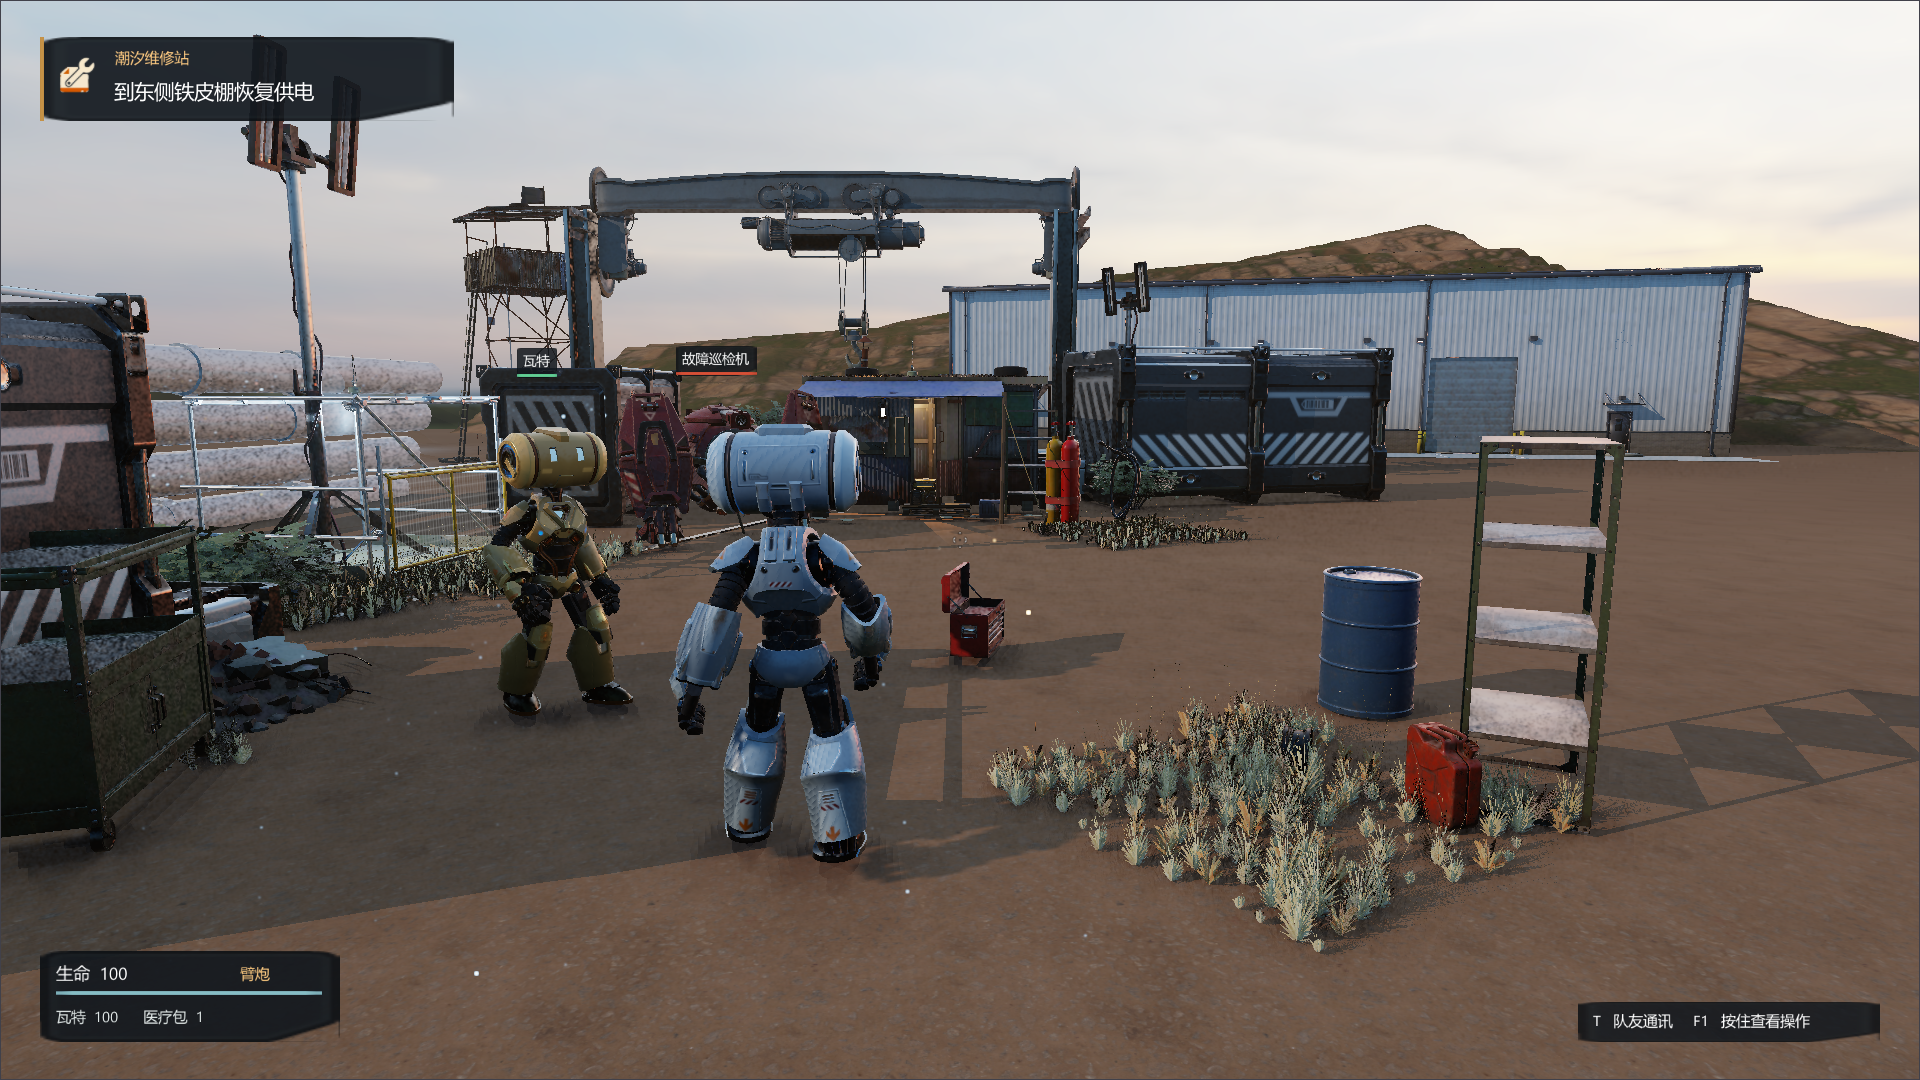
\includegraphics[width=\linewidth]{../../../output/validation/watt-station/hud/redesigned/game.png}}{带底板的布局}\hfill
\panelimage{.488\linewidth}{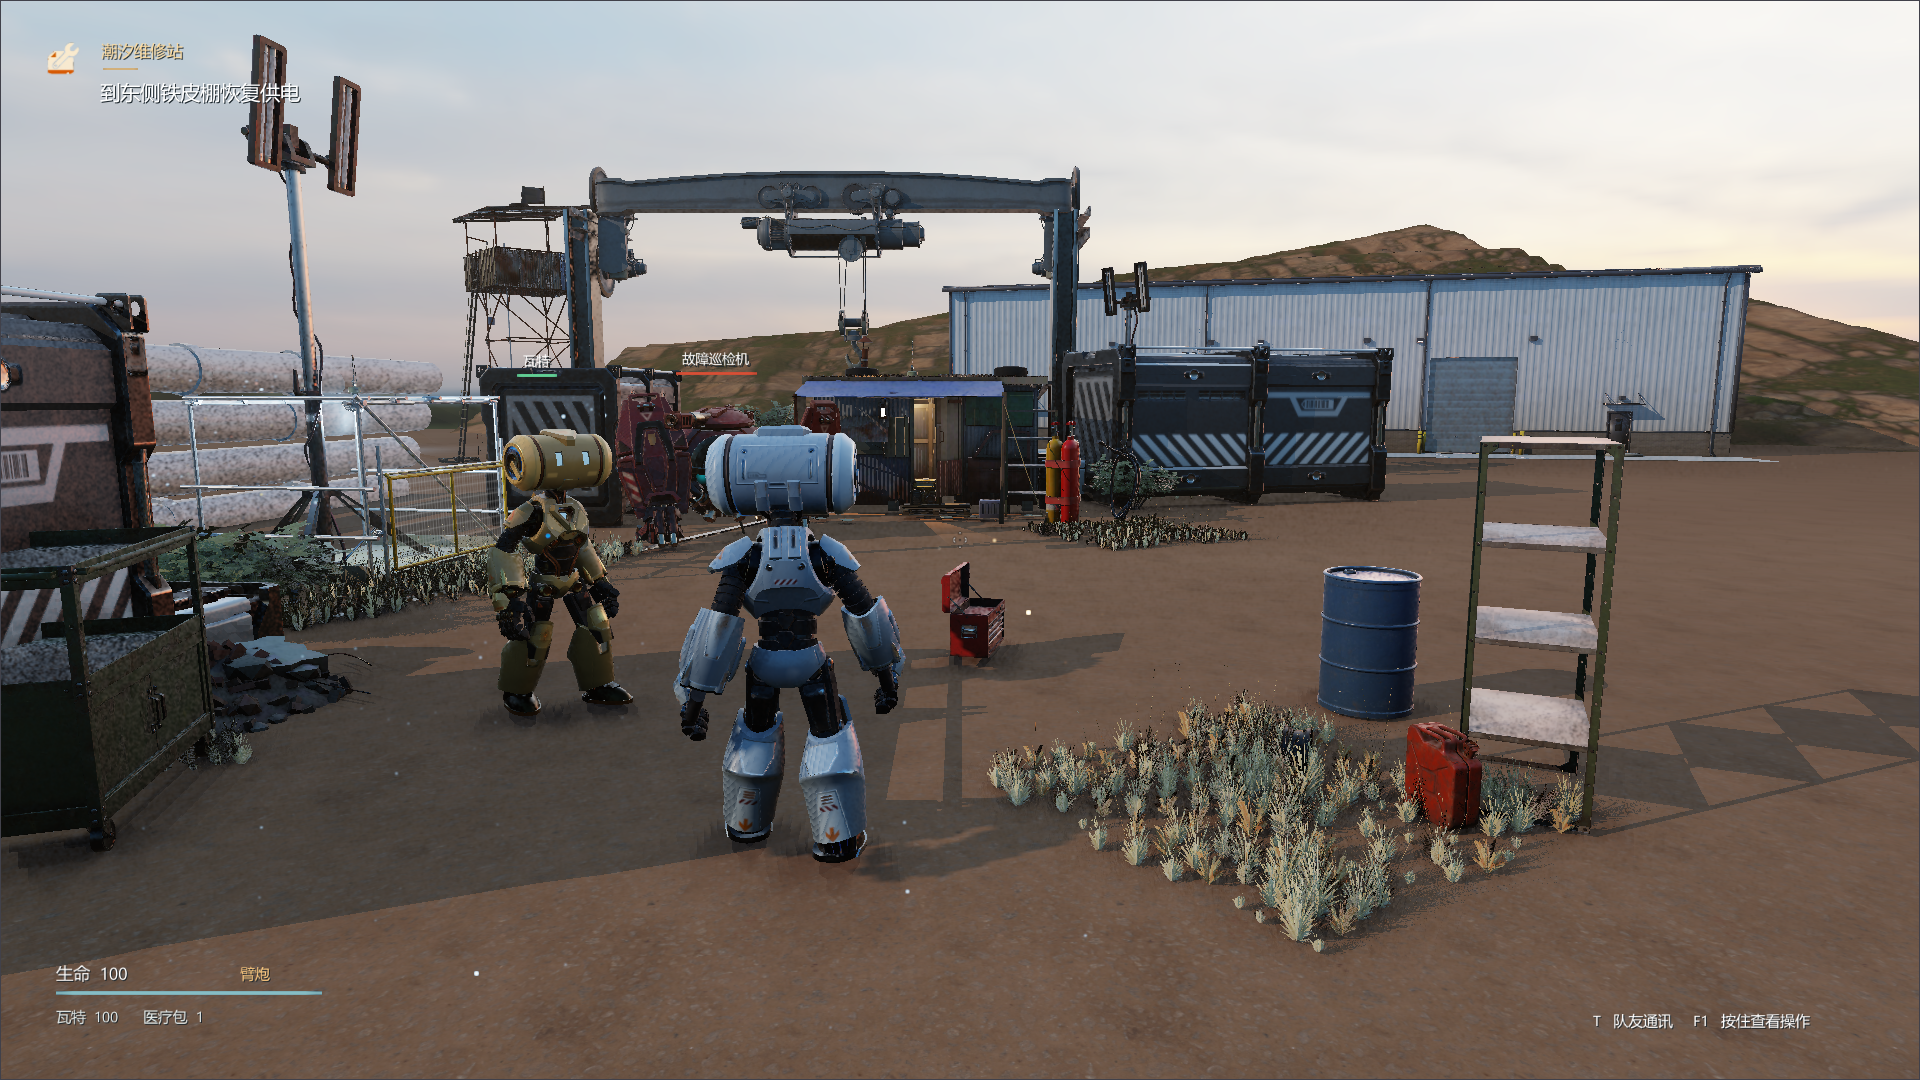
\includegraphics[width=\linewidth]{../../../output/validation/watt-station/hud/final/game.png}}{去掉底板，文字添加字影}
\smallskip

\panelimage{.488\linewidth}{
\includegraphics[width=\linewidth]{../../../output/validation/watt-station/hud/redesigned/coverage.png}}{原布局的覆盖范围}\hfill
\panelimage{.488\linewidth}{
\includegraphics[width=\linewidth]{../../../output/validation/watt-station/hud/final/coverage.png}}{新版布局的覆盖范围}
\end{center}

下排从实际绘制的三角形重建。深灰色没有画界面，青色经过一次，橙色经过两次，红色经过三次或更多。一个字和它的影子可以落在同一像素，因此同一位置可能多次执行片元着色器。每张图左上方都能看到这一区别。

{\smalltable\noindent\begin{tabularx}{\linewidth}{@{}Xrrrr@{}}\toprule
维修站开场，第 12 帧 & HUD 绘制 & 占到的像素 & 片元调用 & 全透明采样\\\midrule
最初布局 & 14 & 145\,876 & 162\,501 & 5\,038\\
任务与状态分区，带底板 & 17 & 78\,186 & 95\,073 & 6\,090\\
文字带字影，移除底板 & 11 & 16\,616 & 29\,191 & 7\,481\\\bottomrule
\end{tabularx}}

在 $1920\times1080$ 的窗口中，新界面占到 0.80\% 的像素。表中的片元调用数直接取自 RenderDoc。最后一列是按字体或图标的 UV 对纹理做双线性采样后得到的估算，全透明处仍可能执行着色器。这解释了字影加入后最后一列增大、总绘制量却明显下降的现象。

\clearpage
\subsection{游戏画面后面的窗口底色}

Vulkan 先清除交换链图像，再由 ImGui 把场景颜色图铺进游戏窗口，最后画文字与图标。检查回放时，场景图之前还有一次绘制。它先把整个窗口涂上主题底色，再画细边框。在铺满窗口的帧里，场景图紧接着覆盖了底色。

修改在 \path{RedflagForge/src/VulkanForgeLayer.cpp} 的 \code{DrawViewport}。独立游戏窗口先按游戏宽高比求出画面四周的余量。横、纵余量都为零时，把 ImGui 窗口底色的透明度设为零，边框照常绘制。缩成 $1200\times900$ 时，上下两条未被场景图覆盖，仍由原来的主题底色填满。Vulkan 的清屏保持在 \code{VulkanContext::BeginWindowPass}。

{\smalltable\noindent\begin{tabularx}{\linewidth}{@{}Xrrr@{}}\toprule
画幅与状态 & 窗口底色和边框 & 场景图 & HUD\\\midrule
$1920\times1080$，原窗口 & 2\,085\,584 & 2\,067\,604 & 162\,501\\
$1920\times1080$，省去底色 & 11\,984 & 2\,067\,604 & 162\,501\\
$1200\times900$，修改前和修改后 & 1\,088\,384 & 808\,650 & 63\,539\\\bottomrule
\end{tabularx}}

表中均为 RenderDoc 的实际片元计数。前两行用了同一版本的 HUD、脚本及场景，显卡少画的 $2\,073\,600$ 个片元正好等于窗口面积。画场景图的四个顶点、UV 和裁切矩形完全相同。两条黑边中取到的 260\,728 个像素逐像素相同。游戏内正在播放的动作会随运行时间前进，比较时没有用角色轮廓充当静止参照。

在 GeForce RTX 5070 Ti Laptop GPU 上测 Debug 版，每份帧先回放一次，再取 11 次 GPU 事件耗时的中位数。原窗口底色和边框是 0.0171 毫秒，省去底色后是 0.0040 毫秒。引擎的 CPU 记录取第 17 至 56 帧，\code{ImGuiLayer::End} 的中位数分别为 155.5 和 167.0 微秒。这个范围涵盖界面绘制数据整理及 Vulkan 命令录制，队列提交在别处。该组 CPU 时间没有随片元数下降。

从仓库根目录运行下面的命令。测试分别捕获带 HUD 和移除 HUD 的一帧，在后一帧定位窗口与场景图，再到前一帧读出额外的 HUD 绘制。

\begin{lstlisting}
python tests/check_game_hud.py --label current --timing
\end{lstlisting}

加上 \code{--window 1200 900} 可以检查带黑边的窗口。三版截图、几何覆盖图、事件号、构建和帧文件哈希保存在 \path{output/validation/watt-station/hud/}。上述结果适用于维修站开场时显示的内容。

\clearpage
\section{维修站的游戏分辨率}

玩家默认看到 $1920\times1080$ 的场景。在帧率较低的电脑上，可以双击
\code{Play-720p.cmd}，也可以运行 \code{Play.cmd --render-size 1280x720}。
此时三维场景先画到一张 $1280\times720$ 的图上，显示时铺满原来的窗口。准星、文字和血条仍按窗口的 $1920\times1080$ 像素绘制，两种设置下的按钮位置相同。

在维修站出生点保持主相机不动，用同一份 Windows x64 Release 程序交替运行四次，顺序是 1080p、720p、720p、1080p。每次跳过起初 15 帧，记录第 16 到 60 帧，每个分辨率共得到 90 个帧间隔。位置按毫米核对，四轮均无输入。下表使用实际游玩时记录的相邻帧间隔，单位为毫秒，涵盖游戏逻辑、绘制和显示等待。

\begin{center}
\begin{tabular}{lrrr}\toprule
场景分辨率 & 场景像素数 & 中位帧时间 & P95 帧时间\\\midrule
$1920\times1080$ & 2\,073\,600 & 87.77 & 93.86\\
$1280\times720$  &   921\,600 & 58.12 & 64.76\\\bottomrule
\end{tabular}
\end{center}

这台 RTX 5070 Ti Laptop GPU 在该机位每帧节省了约 29.65 毫秒。720p 仍高于每秒 60 帧所需的 16.67 毫秒。计时结束后，另用 RenderDoc 1.47 捕获两份第 12 帧。两个版本的同一次网格绘制各使用 6144 个索引，默认设置在事件 185 写入两张 $1920\times1080$ 的表面图，720p 在事件 186 将它们写成 $1280\times720$。最后的界面绘制分别位于事件 2473 和 2474，两者写入的窗口图都是 $1920\times1080$。

可从仓库根目录运行 \path{tests/check_player_resolution.py} 并传入游戏压缩包复测。指定 \code{--renderdoc} 和工具目录可回读上述附件。每帧耗时、相机位置、附件格式和捕获文件哈希保存在 \path{output/validation/packaged-watt/resolution*.json}。帧间隔无法单独给出 GPU 的执行时间，其他机位或设备需要另测。
